\selectlanguage{english}

\section{Schwarzschild black holes}

The simplest black hole solution is the Schwarzschild metric:
\begin{equation}
  ds^2 = - \left( 1 - \frac{2GM}{r} \right) dt^2 + \left( 1 - \frac{2GM}{r} \right)^{-1} dr^2 + r^2 \left( d\vartheta^2 + \sin^2 \vartheta\, d\varphi^2 \right)
  \label{eq:6.1}
\end{equation}
This is a special case of the general metric in Sec. \ref{ds-space} with $ f(r)^2 = 1 - 2GM / r $: it solves the vacuum Einstein equations $ R_{\mu \nu} = 0 $.\\
This solution depends on a single parameter $ M $, which is identified as the mass of the black hole: from the Newtonian approximation $ g_{00} = - (1 + 2\Phi) $, so $ \Phi = - \frac{GM}{r} $, which is precisely the potential for a point mass $ M $ at the origin. The same can be shown via Komar integrals: note that the Schwarzschild metric admits a timelike Killing vector field $ K = \pa_t $, with dual 1-form $ K = g_{00} dt $ and 2-form:
\begin{equation*}
  F = dK = - \frac{2GM}{r^2} dr \wedge dt
\end{equation*}
The associated Komar charge is:
\begin{equation*}
  M_{\text{Komar}} = - \frac{1}{8\pi G} \int_{\mathbb{S}^2_R} \star\, F = M
\end{equation*}
for all $ R > 2GM $ (radius of the horizon). Although the 2-form $ F $ obeys the vacuum Maxwell equations $ d\star F = 0 $, thus one would expect the associated Komar charge to vanish as there's no current, $ M_{\text{Komar}} = M \neq 0 $: this is possible because the mass of the black hole is localized at the origin, where $ F $ diverges. Moreover, the Schwarzschild solution is mathematically valid for $ M \in \R $: the solution $ M = 0 $ is just Minkowski spacetime, while $ M < 0 $ will be shown to be unphysical.

\subsection{Birkhoff theorem}

\begin{theorem}[Birkhoff]
  The Schwarzschild solution is the unique spherically-symmetric and asimptotically-flat solution to the vacuum Einstein field equations.
\end{theorem}
\begin{proof}
  First, spherical symmetry means that the metric has an $ \SOn{3} $ isometry. It can be shown that any metric with such isometry can be written as:
  \begin{equation*}
    ds^2 = g_{\tau \tau}(\tau, \rho) d\tau^2 + 2 g_{\tau \rho}(\tau, \rho) d\tau\,d\rho + g_{\rho \rho}(\tau, \rho) d\rho^2 + r^2(\tau, \rho) d\Omega_2^2
  \end{equation*}
  These coordinates make the $ \SOn{3} $ isometry manifest, as it acts on $ \mathbb{S}^2 $ leaving $ \tau $ and $ \rho $ unchanged: this is a \textit{foliation} of the space by $ \mathbb{S}^2 $. Being $ r(\tau,\rho) $ the size of the sphere, it is useful to change coordinates to $ \tau $ and $ r $:
  \begin{equation*}
    ds^2 = g_{\tau \tau}(\tau,r) d\tau^2 + 2g_{\tau r}(\tau,r) d\tau\,dr + g_{rr}(\tau,r) dr^2 + r^2 d\Omega_2^2
  \end{equation*}
  Note a subtlety: for some functions $ r(\tau,\rho) $ it's not possible to exchange $ r $ and $ \rho $ (ex.: $ r = \tau $), but these counterexamples are ruled out by the assumption that the spacetime is asymptotically the Minkowski spacetime. Now, to get rid of the cross-term, consider $ \tilde{t}(\tau,r) $:
  \begin{equation*}
    d\tilde{t}^2 = \left( \frac{\pa \tilde{t}}{\pa \tau} \right)^2 d\tau^2 + 2 \frac{\pa \tilde{t}}{\pa \tau} \frac{\pa \tilde{t}}{\pa r} d\tau\,dr + \left( \frac{\pa \tilde{t}}{\pa r} \right)^2 dr^2
  \end{equation*}
  It's always possible to pick $ \tilde{t}(\tau,r) $ such that the cross-term vanishes, so that:
  \begin{equation*}
    ds^2 = - f(\tilde{t},r) d\tilde{t}^2 + g(\tilde{t},r) dr^2 + r^2 d\Omega_2^2
  \end{equation*}
  Solving the Einstein field equations requires that $ f(\tilde{t},r) = h(\tilde{t}) f(r) $ and $ g(\tilde{t},r) = g(r) $, thus redefining $ h(\tilde{t}) d\tilde{t}^2 = dt^2 $ yields:
  \begin{equation*}
    ds^2 = - f(r) dt^2 + g(r) dr^2 + r^2 d\Omega_2^2
  \end{equation*}
  Note that, even though time-independence was not assumed, it was derived from the field equations: this metric has the timelike Killing vector $ K = \pa_t $, besides those from the $ \SOn{3} $ isometry. At this point, the field equations require that $ f(r) = g(r)^{-1} $, thus this metric reduces to that considered in Sec. \ref{geo-ds}: the Schwarzschild metric is the most general solution with $ \Lambda = 0 $.
\end{proof}

Therefore, the Schwarzschild metric does not only describe a black hole, but it describes the spacetime outside any non-rotating spherically-symmetric object, even in the presence of time-dependence (ex.: collapsing star).

\begin{definition}\label{def-t-ind}
  A spacetime is said to be \textit{stationary} if it admits a globally-timelike Killing vector field $ K $. In addition, being $ t $ the coordinate along the integral curves of $ K $, if it is invariant under $ t \rightarrow -t $, then it is said to be \textit{static}.
\end{definition}

The definition of static spacetime rules out $ dt dx $ cross-terms in the metric.

\begin{proposition}
  A spherically-symmetric metric must be static.
\end{proposition}
\begin{proof}
  By Birkhoff theorem.
\end{proof}

\subsection{Horizon}

The Schwarzschild metric diverges at $ r = 0 $ and $ r = 2GM \equiv R_s $. To distinguish between true singularities and coordinate singularities, the usual way is defining a coordinate-independent scalar quantity and studying it at divergence points.\\
Due to the vacuum field equations, the simplest scalars $ R $ and $ R_{\mu \nu} R^{\mu \nu} $ both vanish: the next simplest curvature scalar is the \textit{Krentschmann scalar} $ R^{\mu \nu \rho \sigma} R_{\mu \nu \rho \sigma} $, which for the Schwarzschild metric is:
\begin{equation}
  R^{\mu \nu \rho \sigma} R_{\mu \nu \rho \sigma} = \frac{48 G^2 M^2}{r^6}
  \label{eq:6.2}
\end{equation}
At $ r = 2GM $, the Krentschmann scalar is $ \sim 1 / (GM)^4 $, suggesting that this is only a coordinate singularity: it turns out that's the case, and indeed the surface $ r = R_s $ is known as the \textit{event horizon} of the black hole. Note that, interestingly, heavier black holes have smaller curvature at the horizon.\\
On the contrary, $ r = 0 $ is a true singularity, simply known as the \textit{singularity} of the (classical) black hole.

\subsubsection{Near horizon limit}

To study the spacetime in the vicinity of the horizon, set $ r = 2GM + \eta $, with $ \abs{\eta} \ll 2GM $. Moreover, consider $ \eta \in \R^+ $, thus restricting to the spacetime just outside the horizon. The metric then becomes at first order in $ \eta $:
\begin{equation*}
  ds^2 = - \frac{\eta}{2GM} dt^2 + \frac{2GM}{\eta} d\eta^2 + (2GM)^2 d\Omega_2^2
\end{equation*}
Spacetime is thus decomposed in a direct product of $ \mathbb{S}^2_{2GM} $ and a 2d Lorentzian manifold. Focusing on the latter, set $ \rho^2 = 8GM \eta $, so that:
\begin{equation}
  ds^2 = - \left( \frac{\rho}{4GM} \right)^2 dt^2 + d\rho^2
  \label{eq:6.3}
\end{equation}
This is called \textit{Rindler metric} and it is, in fact, just Minkowski spacetime:
\begin{equation*}
  T = \rho \sinh \left( \frac{t}{4GM} \right)
  \qquad
  X = \rho \cosh \left( \frac{t}{4GM} \right)
  \quad \Rightarrow \quad
  ds^2 = - dT^2 + dX^2
\end{equation*}
These are precisely the coordinates Eqq. \ref{eq:1.33}-\ref{eq:1.34} experienced by an observer undergoing constant acceleration $ a = 1 / (4GM) $: this makes sense, as an observer sitting at constant $ \rho $, i.e. constant $ r $, must accelerate in order not to fall into the black hole.\\
The outside of the black hole is $ (\rho,t) \in \R^+ \times \R $, corresponding to $ X > \abs{T} $. The horizon $ \rho = 0 $, instead, is mapped to the origin $ T = X = 0 $ of Minkowski space. However, note that the time coordinate is undefined at the origin since $ g_{00} = 0 $: scaling $ t \rightarrow \infty $ and $ \rho \rightarrow 0 $ keeping $ \rho e^{\pm t / 4GM} $ fixed makes it clear that the horizon actually corresponds to the lines:
\begin{equation*}
  r = 2GM \quad \Rightarrow \quad X = \pm T
\end{equation*}
Therefore, the event horizon is not a timelike surface (like the surface of a star), but a null surface.\\
Although the outside of the event horizon is only described by $ X > \abs{T} $, it is nonetheless possible to extend the metric to the whole Minkowski space $ X,T \in \R $: this makes it clear that the event horizon is not a real singularity, as nothing particular happens at $ X = \pm T $ (see Fig. \ref{rindler}). Zooming out, however, the peculiar properties of the horizon start to emerge from a global perspective.

\begin{figure}[b]
  \centering
  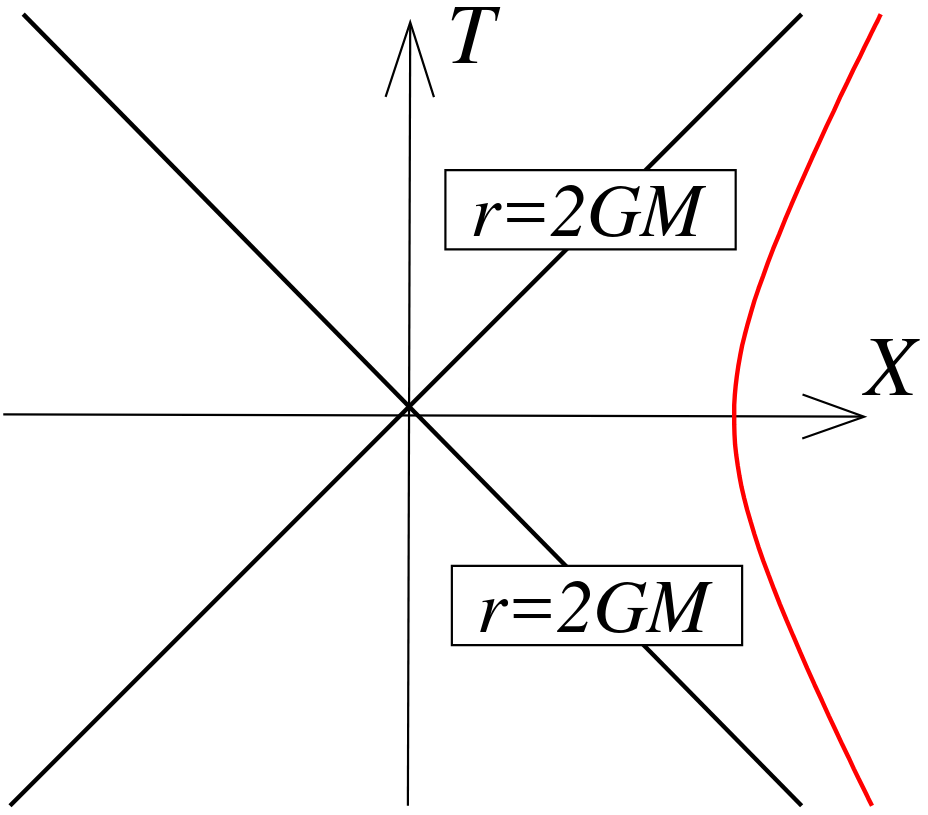
\includegraphics[width = 0.35 \textwidth]{rindler.png}
  \caption{Rindler spacetime, with null lines in black and a line at constant $ r > 2GM $ in red.}
  \label{rindler}
\end{figure}

\subsection{Eddington-Finkelstein coordinates}

Both the Schwarzschild coordinates and the Rindler coordinates do not cover the whole manifold. To find a set of coordinates that does, first introduce a new radial coordinate:
\begin{equation}
  dr_*^2 = \left( 1 - \frac{2GM}{r} \right)^{-2} dr^2
  \quad \Rightarrow \quad
  r_* = r + 2GM \log \left( \frac{r - 2GM}{2GM} \right)
  \label{eq:6.4}
\end{equation}
This is the \textit{Regge-Wheeler radial coordinate} and it maps the region outside the horizon $ r \in (2GM, \infty) $ to $ r_* \in \R $: as an observer approaches the horizon, $ r $ changes increasingly slow varying $ r_* $, since $ \frac{dr}{dr_*} \rightarrow 0 $ as $ r \rightarrow 2GM $. This coordinate is suited to describe the path of lightrays travelling in the radial direction:
\begin{equation*}
  ds^2 = 0
  \quad \Rightarrow \quad
  \frac{dr}{dt} = \pm \left( 1 - \frac{2GM}{r} \right)
  \quad \Rightarrow \quad
  \frac{dr_*}{dt} = \pm 1
  \quad \Rightarrow \quad
  t \pm r_* = \text{const.}
\end{equation*}
These null radial geodesics correspond to an ingoing lightray for the positive sign and an outgoing lightray for the negative sign ($ r_* $ must decrease/increase as $ t $ increases). Next, introduce a pair of null coordinates:
\begin{equation}
  v = t + r_*
  \qquad
  u = t - r_*
  \label{eq:6.5}
\end{equation}
These allow to extend the Schwarzschild solution beyond the horizon.

\subsubsection{Ingoing coordinates}

Replace $ t $ with $ t = v - r_*(r) $:
\begin{equation*}
  dt = dv - \left( 1 - \frac{2GM}{r} \right) dr
\end{equation*}
The Schwarzschild metric then becomes, in coordinates $ (v,r) $:
\begin{equation}
  ds^2 = - \left( 1 - \frac{2GM}{r} \right) dv^2 + 2 dv\,dr + r^2 d\Omega_2^2
  \label{eq:6.6}
\end{equation}
This is the Schwarzschild black hole in \textit{ingoing Eddington-Finkelstein coordinates}. Note that there's no more singularity at $ r = 2GM $; however, the $ dv^2 $ term vanishes at the horizon and becomes negative for $ r < 2GM $. Nonetheless, the metric is still non-degenerate thanks to the cross-term:
\begin{equation*}
  \det g = \det
  \begin{bmatrix}
    - (1 - \frac{2GM}{r}) & 1 & 0 & 0 \\
    1 & 0 & 0 & 0 \\
    0 & 0 & r^2 & 0 \\
    0 & 0 & 0 & r^2 \sin^2 \vartheta
  \end{bmatrix}
  = - r^4 \sin^2 \vartheta
\end{equation*}
Thus, the metric is non-degenerate and with Lorentzian signature for all values of $ r \in \R_+ $ (except for the known poles of $ \mathbb{S}^2 $): this means that the radial coordinate can be extended past the horizon. The globally-timelike Killing vector field $ K = \pa_t $ of the Schwarzschild metric is retained in the ingoing Eddington-Finkelstein coordinates as $ K = \pa_v $, however now it is no longer globally-timelike: it remains so outside the horizon, where $ g_{vv} < 0 $, but become spacelike inside it, where $ g_{vv} > 0 $. This means that the full black hole geometry is not time-independent.\\
Recall that ingoing lightrays follow geodesics given by $ v = \text{const.} $, while outgoing lightrays follow $ u = t - r_* = \text{const.} $. As a function of $ (v,r_*) $, the latter reads $ v = 2r_* + \text{const.} $, so in $ (v,r) $ coordinates:
\begin{equation*}
  v =  2r + 4GM \log \left( \frac{r - 2GM}{2GM} \right) + \text{const.}
\end{equation*}
This clearly has domain $ r \in (2GM, \infty) $, therefore the Regge-Wheeler radial coordinate needs a redefinition:
\begin{equation*}
  r_* = r + 2GM \log \abs{\frac{r - 2GM}{2GM}}
\end{equation*}
This means that now $ r_* $ is a multi-valued function: $ r \in (2GM, \infty) $ is mapped to $ r_* \in \R $, while $ r \in (0, 2GM) $ is mapped to $ r_* \in \R_- $, with the singularity at $ r_* = 0 $. Outgoing lightrays inside the horizon will then follow geodesics given by:
\begin{equation*}
  v = 2r + 4GM \log \left( \frac{2GM - r}{2GM} \right) + \text{const.}
\end{equation*}
Outgoing null geodesics at the horizon are easily found: the $ dv^2 $ term in the metric Eq. \ref{eq:6.6} vanishes and the surface $ r = 2GM $ is itself a null geodesic (as event horizons are always null surfaces).

\begin{figure}
  \centering
  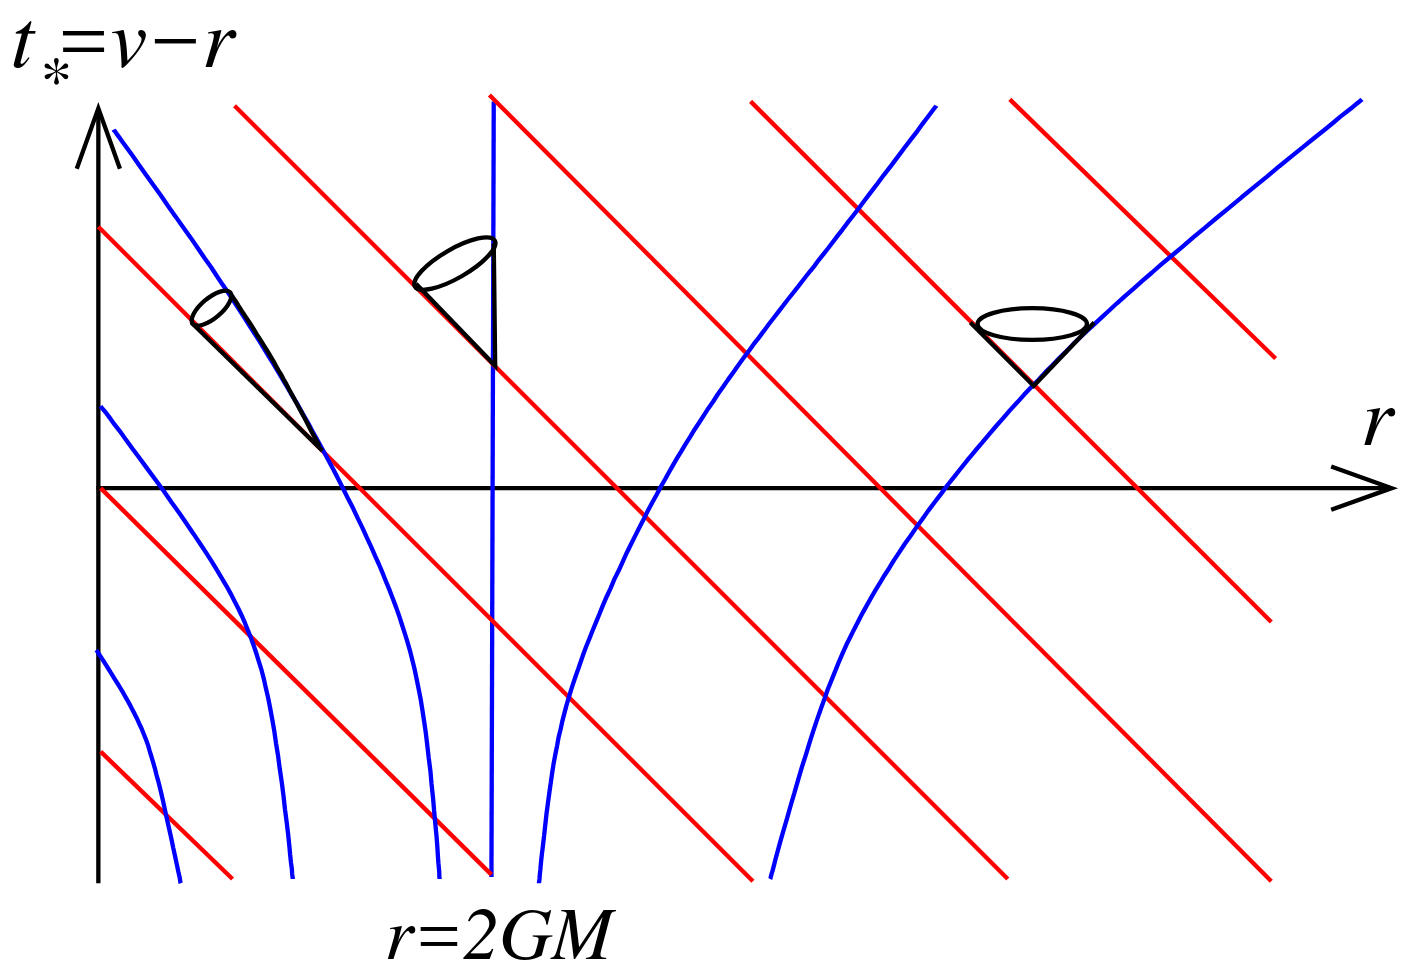
\includegraphics[width = 0.50 \textwidth]{ef-in.png}
  \caption{Finkelstein diagram in ingoing coordinates: ingoing null geodesics are shown in red, outgoing ones in blue.}
  \label{ef-in}
\end{figure}

All of this information about lightrays can be pictured in a \textit{Finkelstein diagram}, which shows null geodesics in a radial-temporal diagram. Since $ r_* $ is multi-valued, $ r $ is chosen as radial coordinate: as a consequence, one needs to define a new temporal coordinate $ t_* : v = t + r_* = r_* + r $, i.e. $ t_* = v - r $. The Finkelstein diagram in ingoing coordinates is shown in Fig. \ref{ef-in}: ingoing null geodesics are $ v = \text{const.} $, i.e. $ t_* = \text{const.} - r $, hence travelling at 45°, while outgoing ones are given by the previously found expressions. Note that only outgoing null geodesics outside of the horizon effectively $ \virgolette{go out} $, since $ r \rightarrow \infty $ as $ t \rightarrow \infty $ (so $ t_* \rightarrow \infty $): those inside the horizon move inexorably towards the curvature singularity at $ r = 0 $ as time passes, and each one of them reaches it in a finite time $ t_* $. The boundary between these two regions are the null geodesics which run along the horizon at $ r = 2GM $.\\
This analysis can be extended to massice particles: they must move along timelike geodesics inside their future lightcone, which is determined by a pair of ingoing and outgoing future-pointing null geodesics. These future lightcones are also shown in Fig. \ref{ef-in}: the name $ \virgolette{black hole} $ captures the causal structure of the spacetime, as neither massive particles nor lightrays can escape outside of the event horizon, thus an outside observer can know nothing of the inside of the black hole.\\
Consider two observers, one at constant $ r > 2GM $ and the other moving towards the singularity: as the second approaches the event horizon, light signals emitted by it will take longer and longer to reach the first, and they will appear progressively more redshifted due to the increasingly strong gravitational well. Thus, the outside observer will see the ingoing observer forever, but progressively more slowed down and redshifted, and will never see it passing the event horizon.

\subsubsection{Outgoing coordinates}

A different extension of the exterior of the Schwarzschild black hole is obtained by replacing $ t $ with $ u = t - r_* $, i.e. $ t = u + r_*(r) $:
\begin{equation}
  ds^2 = - \left( 1 - \frac{2GM}{r} \right) du^2 -2 du\,dr + r^2 d\Omega_2^2
  \label{eq:6.7}
\end{equation}
This is the Schwarzschild black hole in \textit{outgoing Eddington-Finkelstein coordinates}. Once again, the metric is smooth and non-degenerate at the horizon, thus it's possible to extend $ r \in \R_+ $. However, now $ r \in (0,2GM) $ describe a different part of spacetime from the analogous region in ingoing coordinates. To see this, set coordinates $ (r,t_*) : t_* = u + r $ and draw the Finkelstein diagram (Fig. \ref{ef-out}): outgoing null geodesics hence travel at 45°, effectively $ \virgolette{going out} $ regardless of their position with respect to the horizon. On the contrary, ingoing null geodesics now don't $ \virgolette{go in} $: those starting outside of the horizon pile up at the horizon itself, unable to cross it, while those starting inside the horizon move outwards and pile up at it, still unable to cross it.

\begin{figure}
  \centering
  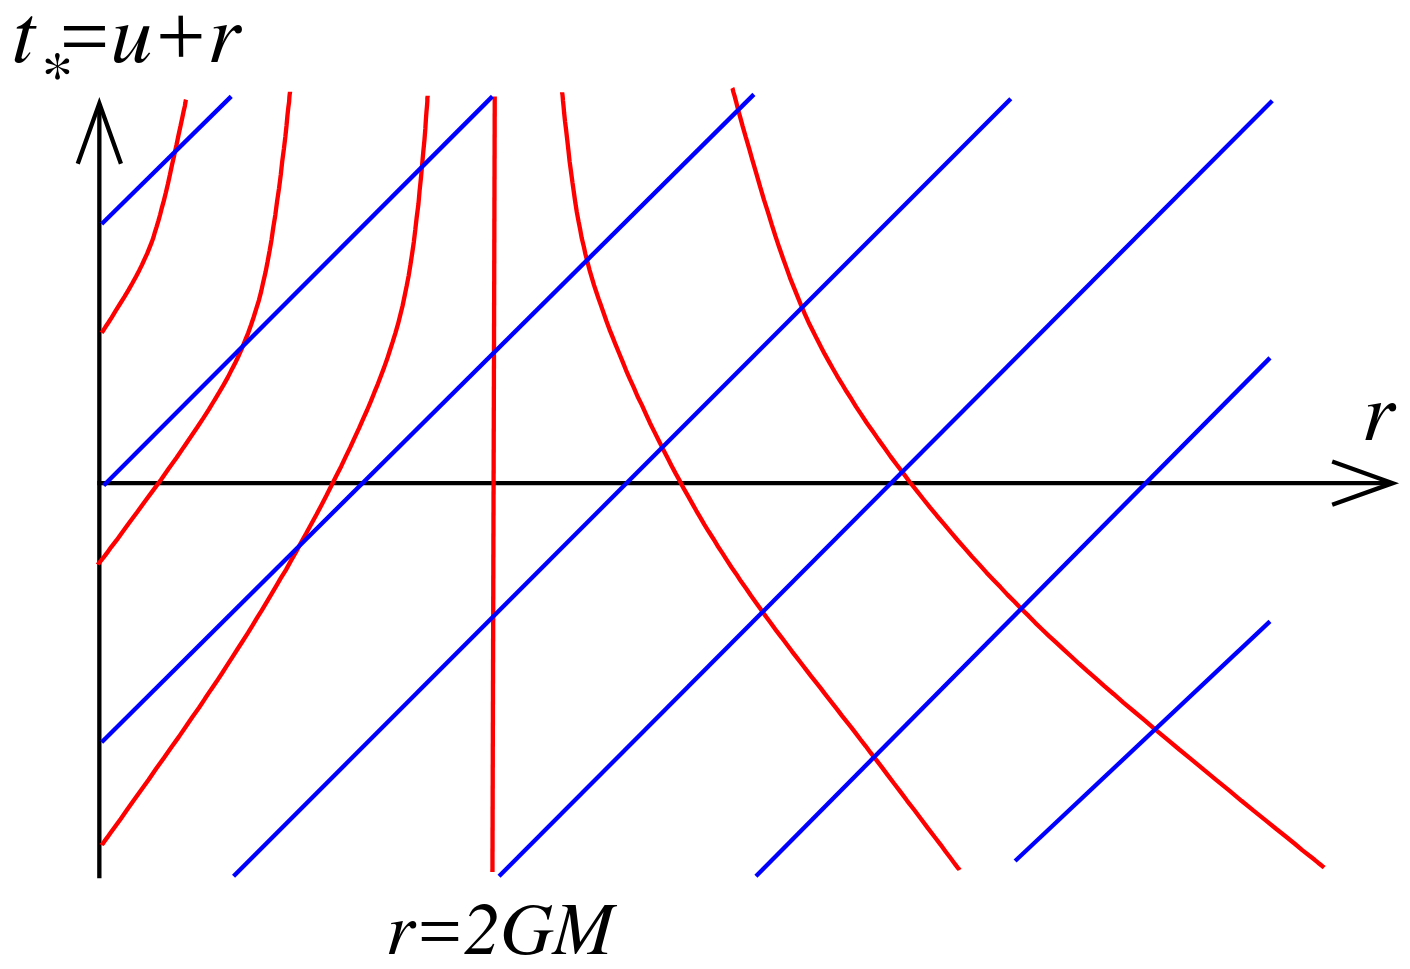
\includegraphics[width = 0.50 \textwidth]{ef-out.png}
  \caption{Finkelstein diagram in outgoing coordinates: ingoing null geodesics are shown in red, outgoing ones in blue.}
  \label{ef-out}
\end{figure}

Studying lightcones, it's easy to see that massive particles inside the horizon are inexorably expelled outside of it in a finite amount of time $ t_* $. This is clearly a very different physics from a black hole: the metric Eq. \ref{eq:6.7} is that of a \textit{white hole}, an object which expells any matter inside. A white hole can be viewed as the time reversal of a black hole: this is to be traced to the negative sign in the cross-term and can be seen by flipping Fig. \ref{ef-out} upside-down, getting Fig. \ref{ef-in}.\\
White holes are perfectly acceptable solutions to the Einstein field equations, and their existence is to be expected from the time-reversal invariance of the field equations. However, they're not physically relevant, as they cannot be formed from collapsing matter.

\subsection{Kruskal spacetime}

To better understand how the region parametrized by $ r \in (0, 2GM] $ corresponds to two different parts of spacetime, one needs to introduce coordinates which cover the entire spacetime, including both black and white holes.\\
First, rewrite the Schwarzschild metric in $ (u,v) $ coordinates:
\begin{equation*}
  ds^2 = - \left( 1 - \frac{2GM}{r} \right) du\,dv + r^2 d\Omega_2^2
\end{equation*}
where $ r = r(u - v) $. There's a degeneracy at $ r = 2GM $ which can be solved introducing the \textit{Kruskal-Szekeres coordinates}:
\begin{equation}
  U = - \exp \left( - \frac{u}{4GM} \right)
  \qquad
  V = \exp \left( \frac{v}{4GM} \right)
  \label{eq:6.8}
\end{equation}
Both $ U $ and $ V $ are null coordinates, and the exterior of the Schwarzschild balck hole is parametrized by $ U < 0, V > 0 $. The metric becomes:
\begin{equation}
  ds^2 = - \frac{32 (GM)^3}{r} e^{-\frac{r}{2GM}} dU\,dV + r^2 d\Omega_2^2
  \label{eq:6.9}
\end{equation}
This is known as the metric of \textit{Kruskal spacetime}. The function $ r = r(U,V) $ can be found inverting:
\begin{equation}
  UV = - \exp \left( \frac{r_*}{2GM} \right) = \frac{2GM - r}{2GM} \exp \left( \frac{r}{2GM} \right)
  \label{eq:6.10}
\end{equation}
On the other hand, the function $ t = t(U,V) $ can be found inverting:
\begin{equation}
  \frac{U}{V} = - \exp \left( - \frac{t}{2GM} \right)
  \label{eq:6.11}
\end{equation}
The original Schwarzschild metric, which covers $ U < 0, V > 0 $, can now be extended to $ (U,V) \in \R^2 $, without any divergence at $ r = 2GM $.

\begin{proposition}
  Kruskal spacetime is the \textit{maximal extension} of the Schwarzschild metric.
\end{proposition}
\begin{proof}
  To check whether a given spacetime can be further extended, one needs to look at all possible geodesics: if they are defined for infinite affine parameter, then they can escape to infinity; however, if they alt at some finite affine parameter, that is either a coordinate singularity, hinting that the spacetime can in fact be extended, or a true singularity. A spacetime is maximally extended if any geodesics that alts at a finite affine parameter does so at a true singularity, and that's the case for Kruskal spacetime.
\end{proof}

The extension process allows to solve the field equations in some particular region (open subset) of spacetime: being the metric components real analytic functions, this is sufficient to determine the metric in all of spacetime.

\subsubsection{Kruskal diagram}

To see where the event horizon is mapped in Kruskal spacetime:
\begin{equation*}
  r = 2GM
  \qquad \Rightarrow \qquad
  U = 0 \quad \lor \quad V = 0
\end{equation*}
This means that the event horizon no longer is a null surface, but two null surfaces intersecting at $ U = V = 0 $, in agreement with the near horizon limit (Rindler space): the null surface $ U = 0 $ is the horizon of the black hole, known as the \textit{future horizon}; the null surface $ V = 0 $ is the horizon of the white hole, known as the \textit{past horizon}.
On the other hand, the singularity becomes:
\begin{equation*}
  r = 0
  \qquad \Rightarrow \qquad
  UV = 1
\end{equation*}
This hyperbola has two disconnected components: one ($ U,V > 0 $) corresponding to the singularity of the black hole and one ($ U,V < 0 $) to the singularity of the white hole.

\begin{figure}
  \centering
  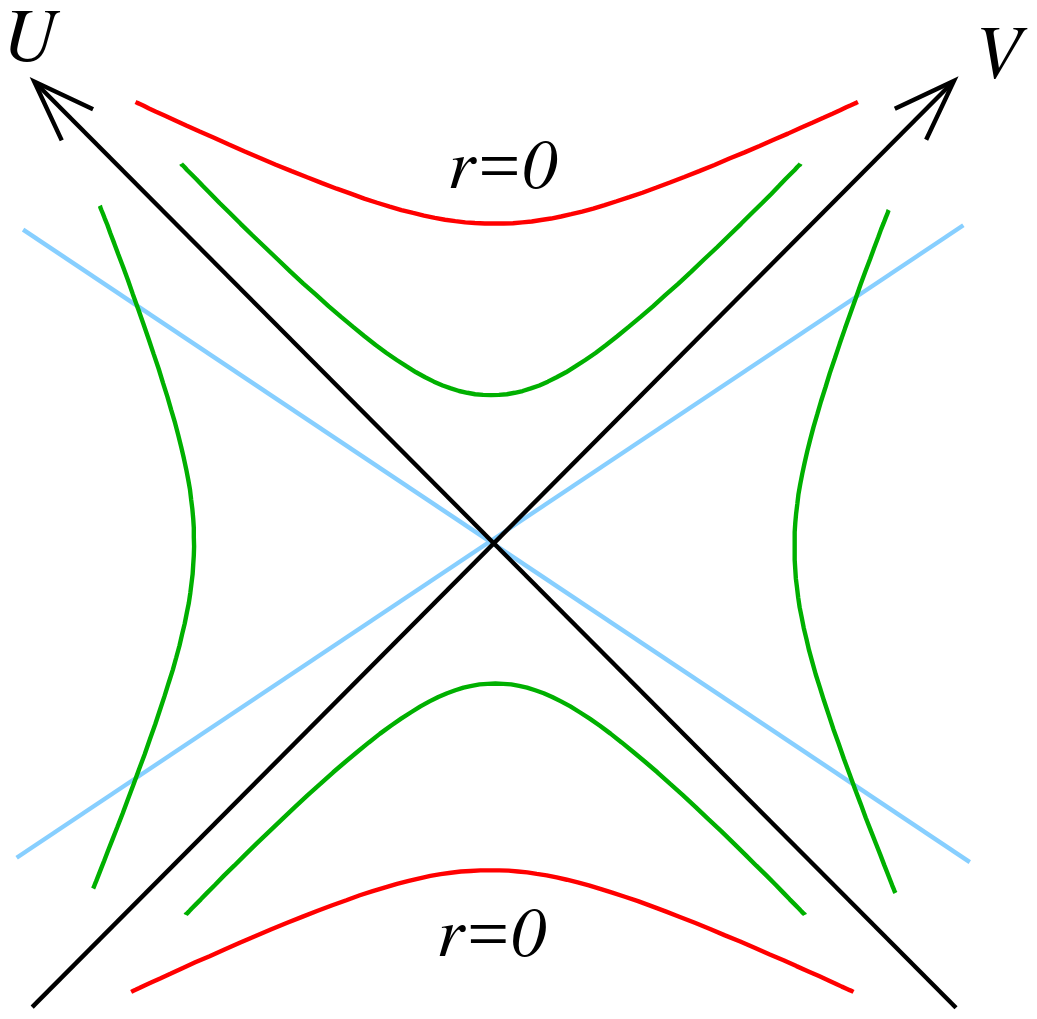
\includegraphics[width = 0.50 \textwidth]{kruskal.png}
  \caption{Kruskal diagram for the Schwarzschild balck hole: green lines are $ r = \text{const.} $ and blue lines $ t = \text{const.} $, while singularities are in red and horizons in black.}
  \label{kruskal}
\end{figure}

All of this information can be represented in a \textit{Kruskal diagram}, as shown in Fig. \ref{kruskal}: the $ U $ and $ V $ axes are at 45°, reflecting that they are null lines, and these are the two horizons. In this diagram, the vertical direction can be viewed as a time coordinate $ T = \frac{1}{2} (V + U) $ and the horizontal one as a spatial coordinate $ X = \frac{1}{2} (V - U) $. This diagram makes it clear that the black hole and the white hole cohabit the same spacetime. Lines of constant $ r $ and $ t $ correspond respectively to lines of constant $ UV $ and $ U/V $, as from Eqq. \ref{eq:6.10}-\ref{eq:6.11}.\\
The Kruskal diagram makes it clear that, once an observer crosses the event horizon, the singularity is unavoidable: the $ r = 0 $ are not timelike worldlines, but \textit{the singularity is spacelike}. Therefore, for the in-falling observer, after crossing the horizon the singularity of the black hole does not lie in a spatial direction, but it lies in the future. Similarly, the singularity of the white hole lies in the past. This can be formally seen using the Killing vector field $ K = \pa_t $ of the Schwarzschild solution. Outside of the horizon $ K $ is timelike, therefore it defines the conserved energy of geodesics; in Kruskal-Szekeres coordinates:
\begin{equation*}
  K = \pa_t = \frac{\pa V}{\pa t} \pa_V + \frac{\pa U}{\pa t} \pa_U = \frac{1}{4GM} \left( V \frac{\pa}{\pa V} - U \frac{\pa}{\pa U} \right)
  \quad \Rightarrow \quad
  g_{\mu \nu} K^\mu K^\nu = - \left( 1 - \frac{2GM}{r} \right)
\end{equation*}
Ouside of the horizon $ K_\mu K^\mu < 0 $ as expected. But inside, with $ r < 2GM $, the Killing vector field is spacelike: therefore, by Def. \ref{def-t-ind}, the full Schwarzschild spacetime is not time-independent, but it becomes clear only after crossing the event horizon.

\paragraph{Einstein-Rosen bridge}

With reference to the Kruskal diagram in Fig. \ref{kruskal}, the right-hand quadrant is the exterior of the black hole, covered by the Schwarzschild coordinates, while the upper and lower quadrants are respectively the interior of the black hole and of the white hole, covered by ingoing and outgoing Eddington-Finkelstein coordinates (see Fig. \ref{kruskal-rind}). There remains the left-hand quadrant: this turns out to be just another copy of the exterior of the black hole, now covered by $ U > 0, V < 0 $.

\begin{figure}
  \centering
  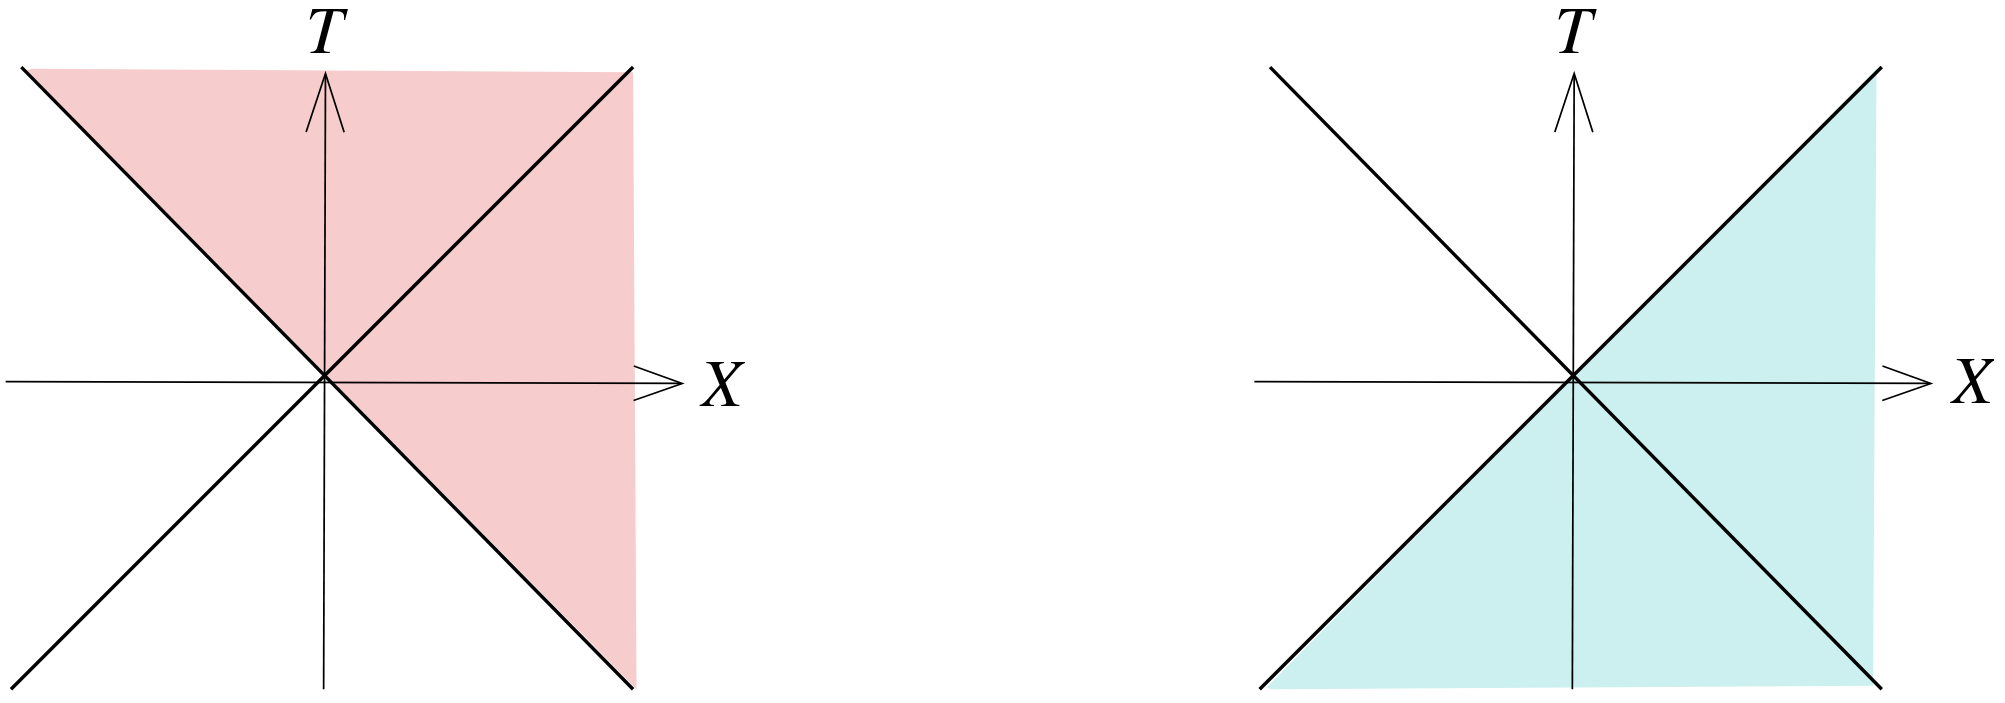
\includegraphics[width = 0.70 \textwidth]{kruskal-rind.png}
  \caption{Regions of Kruskal spacetime covered by ingoing and outgoing Eddington-Finkelstein coordinates respectively.}
  \label{kruskal-rind}
\end{figure}

The full spacetime hence contains two asymptotically flat regions, joined together by a black hole: note that it's not possible for an observer in one region to send a signal in the other, because the causal structure of the spacetime doesn't allow this.\\
To elucidate the spatial geometry connecting these two regions, one need to study the $ t = 0 $ hypersurface of Kruskal spacetime: this is a straight horizontal line passing through $ U = V = 0 $ in Fig. \ref{kruskal}. In Schwarzschild coordinates, the geometry of the $ t = 0 $ hypersurface is given by:
\begin{equation}
  ds^2 = \left( 1 - \frac{2GM}{r} \right)^{-1} dr^2 + r^2 \left( d\vartheta^2 + \sin^2 \vartheta \, d\varphi^2 \right)
  \label{eq:6.12}
\end{equation}
which is valid for $ r > 2GM $. Kruskal spacetime presents two copies of this geometry, one in the right-hand quadrant and one in the left-hand one, which are glues together at $ r = 2GM $ to give a wormhole-like geometry as in Fig. \ref{wormhole}: this is called the \textit{Einstein-Rosen bridge}. Note that it's not possible to travel through it, as the paths are spacelike, not timelike.

\begin{figure}
  \centering
  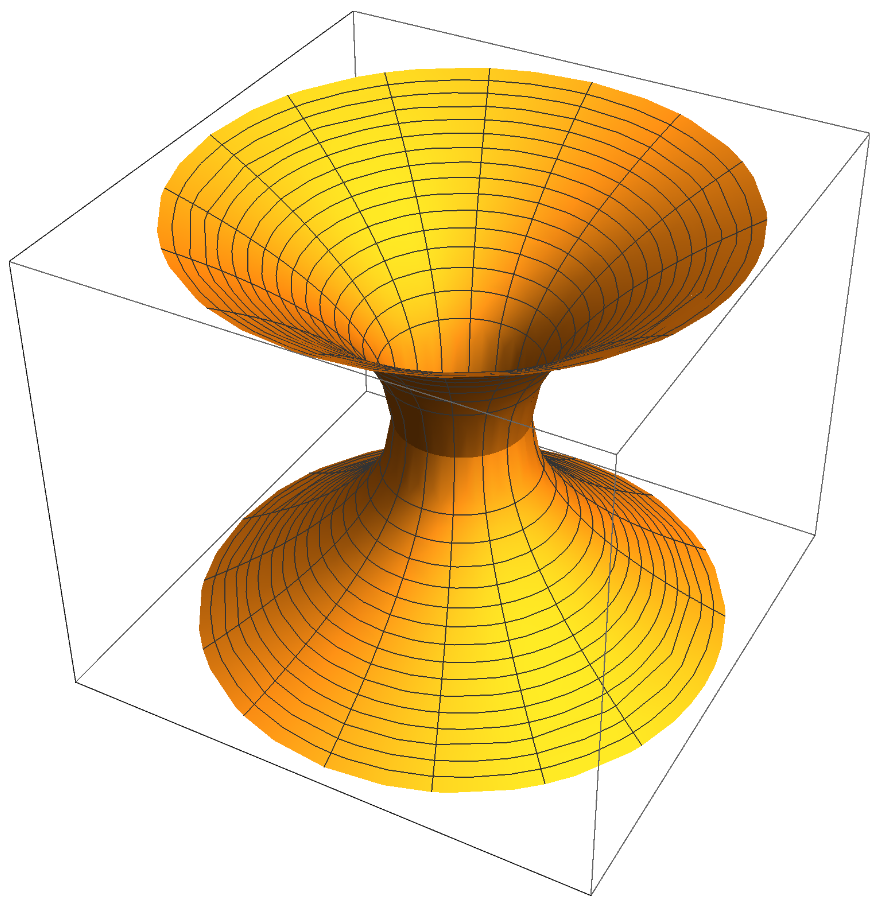
\includegraphics[width = 0.40 \textwidth]{wormhole.png}
  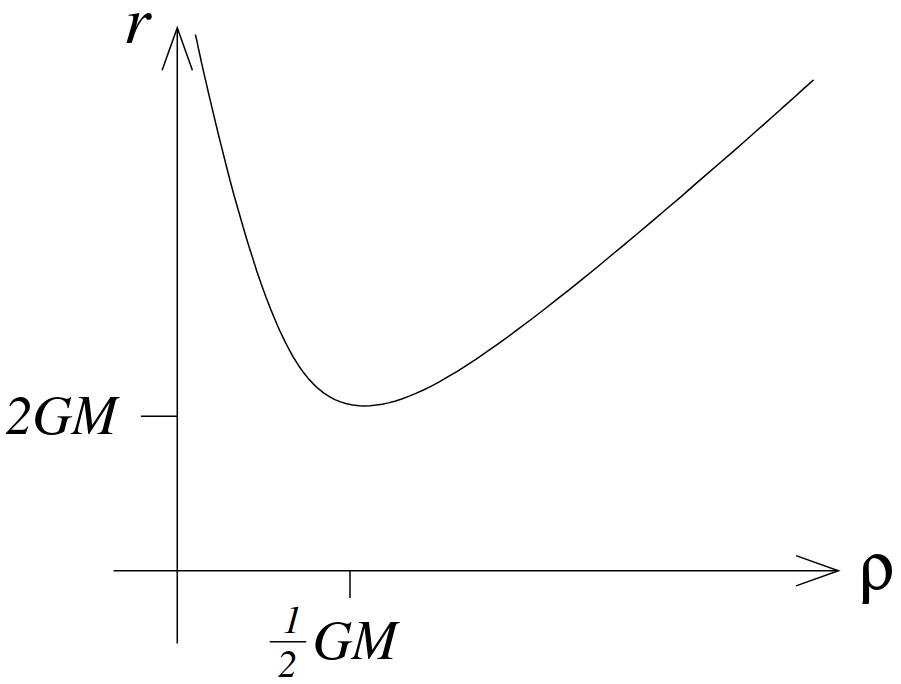
\includegraphics[width = 0.50 \textwidth]{wormhole-rho.png}
  \caption{The Einstein-Rosen bridge and the $ \rho $ coordiante which parametrizes it.}
  \label{wormhole}
\end{figure}

It's possible to write a metric which includes both sides. Define the radial coordinate $ \rho $ such that:
\begin{equation*}
  r = \rho \left( 1 + \frac{GM}{2\rho} \right)^2 = \rho + GM + \frac{G^2 M^2}{4 \rho}
\end{equation*}
Plotting $ r = r(\rho) $, as in Fig. \ref{wormhole}, it's clear that there are two values of $ \rho $ for each value of $ r > 2GM $, while $ r = 2GM $ only corresponds to $ \rho = GM/2 $: thus, is possible to parametrize one side of the wormhole with $ \rho \in (0, GM/2) $ and the other with $ \rho \in (GM/2, \infty) $. The metric in Eq. \ref{eq:6.12} becomes:
\begin{equation}
  ds^2 = \left( 1 + \frac{GM}{2\rho} \right)^4 \left[ d\rho^2 + \rho^2 \left( d\vartheta^2 + \sin^2 \vartheta \, d\varphi^2 \right) \right]
  \label{eq:6.13}
\end{equation}
It is clear that, as $ \rho \rightarrow \infty $, the (spatial) metric is that of $ \R^3 $. But the same is true for $ \rho \rightarrow 0 $: note that there's a symmetry $ r \mapsto r $ for $ \rho \mapsto G^2 M^2 / (4\rho) $, which swaps the two asymptotic spacetimes while leaving the midpoint at $ \rho = GM/2 $ invariant, i.e. it swaps the two sides of the wormhole.\\
Furthermore, the radius of the spatial $ \mathbb{S}^2 $ is minimum at $ 2GM $ in the midpoint $ \rho = GM/2 $ of the wormhole and increases in either direction: this middle point corresponds to the common point $ U = V = 0 $ of the two horizons and is called the \textit{bifurcation sphere}.\\
Although there's no way that an observer in one quadrant can signal an observer in the other quadrant, there's one way for them to communicate: jump into the black hole and meet behind the respective horizons. However, as the white hole is thought to have no physical manifestation, the other universe in the left-hand quadrant of Kruskal space is thought to be a mathematical artifact too.

\subsubsection{Penrose diagram}

From the Kruskal diagram in Fig. \ref{kruskal}, it's easy to draw the Penrose diagram for Kruskal spacetime.

\begin{figure}
  \centering
  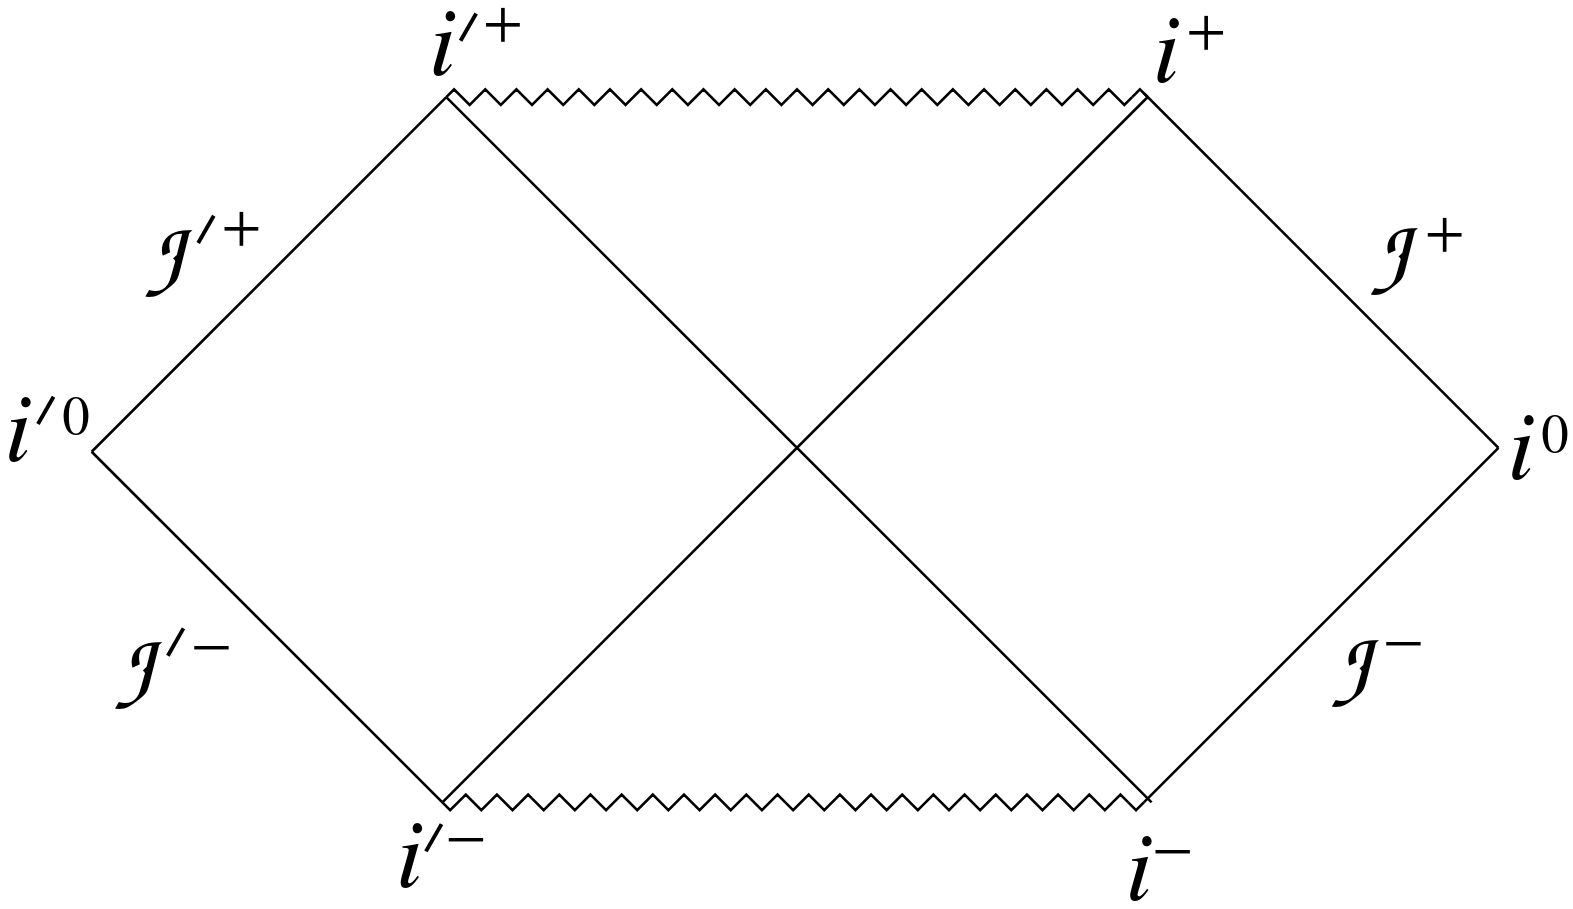
\includegraphics[width = 0.70 \textwidth]{kruskal-penrose.png}
  \caption{The Penrose diagram for Kruskal spacetime.}
  \label{kru-penr}
\end{figure}

First, introduce new coordinates which cover the entire spacetime in a finite range:
\begin{equation*}
  U = \tan \tilde{U}
  \qquad
  V = \tan \tilde{V}
\end{equation*}
The new coordinates have range $ (\tilde{U},\tilde{V}) \in (-\frac{\pi}{2}, + \frac{\pi}{2}) $ and the Kruskal metric becomes:
\begin{equation*}
  ds^2 = \frac{1}{\cos^2 \tilde{U} \, \cos^2 \tilde{V}} \left[ - \frac{32 (GM)^3}{r} e^{-\frac{r}{2GM}} d\tilde{U}\,d\tilde{V} + r^2 \cos^2 \tilde{U} \, \cos^2 \tilde{V} \, d\Omega_2^2 \right]
\end{equation*}
This metric is conformally equivalent to:
\begin{equation*}
  ds^2 = - \frac{32 (GM)^3}{r} e^{-\frac{r}{2GM}} d\tilde{U}\,d\tilde{V} + r^2 \cos^2 \tilde{U} \, \cos^2 \tilde{V} \, d\Omega_2^2
\end{equation*}
However, the singularity at $ r = 0 $ must be retained: this is mapped to $ UV = 1 $, thus in the finite-range coordinates:
\begin{equation*}
  \tan \tilde{U} \, \tan \tilde{V} = 1
  \quad \Leftrightarrow \quad
  \sin \tilde{U} \, \sin \tilde{V} - \cos \tilde{U} \, \cos \tilde{V} = 0
  \quad \Leftrightarrow \quad
  \cos (\tilde{U} + \tilde{V}) = 0
  \quad \Leftrightarrow \quad
  \tilde{U} + \tilde{V} = \pm \frac{\pi}{2}
\end{equation*}
These are straight horizontal lines in the Penrose diagram which chop the diamond-shaped diagram (as that in Fig. \ref{ms-causal}): the resulting diagram is shown in Fig. \ref{kru-penr}, with singularities represented by jagged lines.\\
The Penrose diagram contains the same information as the Kruskal diagram in Fig. \ref{kruskal}, but it allows to state a more rigorous definition of black hole. Restricting to aymptotically flat spacetimes, the two asymptotic regions contain both null infinities $ \mathcal{I}^+ $ and $ \mathcal{I}^- $: the black hole region is then defined as the set of points which cannot send signals to $ \mathcal{I}^+ $. The boundary of the black hole region is the \textit{future event horizon} $ \mathcal{H}^+ $: equivalently, $ \mathcal{H}^+ $ is the boundary of the causal past of $ \mathcal{I}^+ $. With reference to Fig. \ref{kru-penr}, the black hole associated to $ \mathcal{I}^+ $ is the upper quadrant and the left quadrant, while the black hole associated to $ \mathcal{I}'^{+} $ is the upper quadrant and the right quadrant.\\
Importantly, note that to define a black hole one needs to know the whole spacetime, as all lightrays must be run backwards from $ \mathcal{I}^+ $ to determine $ \mathcal{H}^+ $ as their boundary: there's no reference to any spacelike hypersurface at constant coordinate time, thus an observer can't really know if it is inside a black hole unless by knowing the entire future evolution of the spacetime.\\
Equivalently, it's possible to define the white hole region and the \textit{past event horizon} as the region that cannot receive signals from $ \mathcal{I}^- $ and its boundary.

\subsection{Weak cosmic censorship}

Kruskal spacetime is unphysical in a number of ways. In fact, in reality, black holes do not emerge from white holes, but are formed by collapsing stars: the resulting Penrose diagram is rather different from that in Fig. \ref{kru-penr}. To understand the causal structure of such a black hole, consider the (unrealistic) situation of the spherically-symmetric collapse of a shell of matter: inside the shell, spacetime is flat, meanwhile on the outside it is described by Schwarzschild metric Eq. \ref{eq:6.1} (by Birkhoff theorem, time dependence doesn't change this fact). Furthermore, assume (unrealistically) that the shell is travelling at the speed of light, so that the Penrose diagrams for Minkowski spacetime and Kruskal spacetime can be glued as in Fig. \ref{cens-1}: this is the Penrose diagram of a collapsing black hole.

\begin{figure}
  \centering
  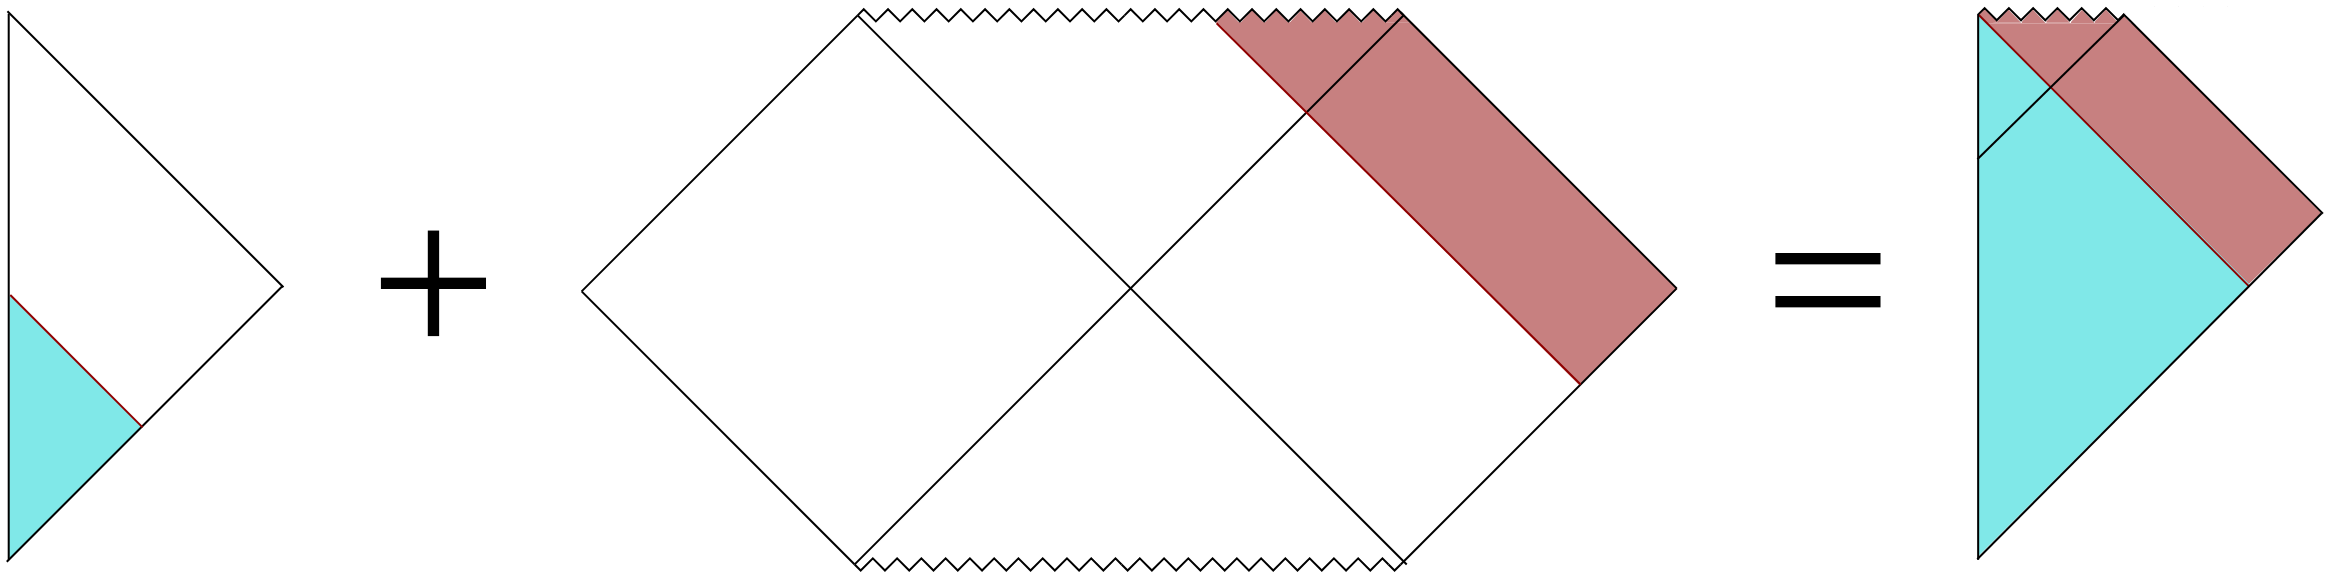
\includegraphics[width = 0.70 \textwidth]{cens-1.png}
  \caption{Joining two Penrose diagrams.}
  \label{cens-1}
\end{figure}

\begin{figure}[b]
  \centering
  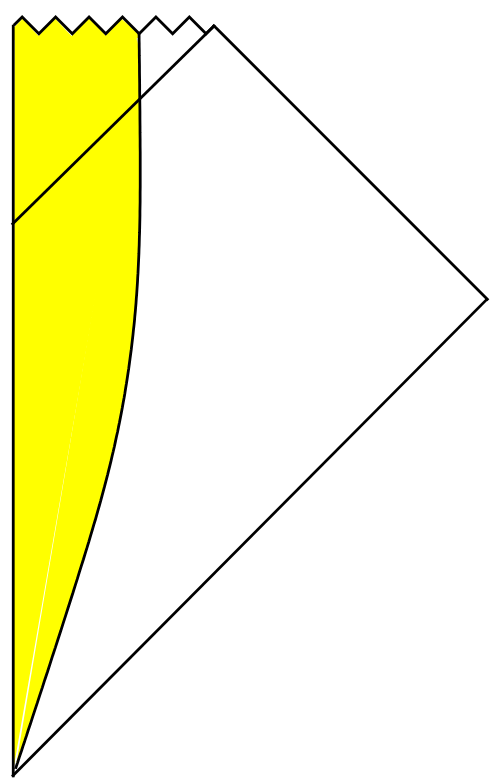
\includegraphics[width = 0.20 \textwidth]{cens-2.png}
  \caption{Penrose diagram for a collapsing star forming a black hole.}
  \label{cens-2}
\end{figure}

Despite the number of unphysical assumptions, the Penrose diagram thus derived correctly describes the causal structure of a realistic spherically-symmetric collapsing star: as in Fig. \ref{eq:6.9}, its surface follows a timelike trajectory.

\subsubsection{Naked singularities}

An important feature of the black hole is that the singularity remains shrouded behind the event horizon, so that an asymptotic observer cannot see it.\\
On the contrary, Einstein field equations also allow \textit{naked singularities}, i.e. singularities without an horizon. For example, consider Schwarzschild metric with $ M < 0 $:
\begin{equation*}
  ds^2 = - \left( 1 + \frac{2G \abs{M}}{r} \right) dt^2 + \left( 1 + \frac{2G \abs{M}}{r} \right)^{-1} dr^2 + r^2 \left( d\vartheta^2 + \sin^2 \vartheta \, d\varphi^2 \right)
\end{equation*}
This metric presents no coordinate singularity at $ r = 2G \abs{M} $, and so no event horizon. The Penrose diagram for such a spacetime is found analogously to that of Minkwoski spacetime (Sec. \ref{sec-penr-mink}), setting null coordinates $ u = t - r $ and $ v = t + r $. The resulting diagram, shown in Fig. \ref{cens-3}, is identical to that of Minkowski spacetime (Fig. \ref{ms-4d}), with the difference that now $ r = 0 $ presents a curvature singularity not shielded by an horizon: it is therefore observed from $ \mathcal{I}^+ $.

\begin{figure}
  \centering
  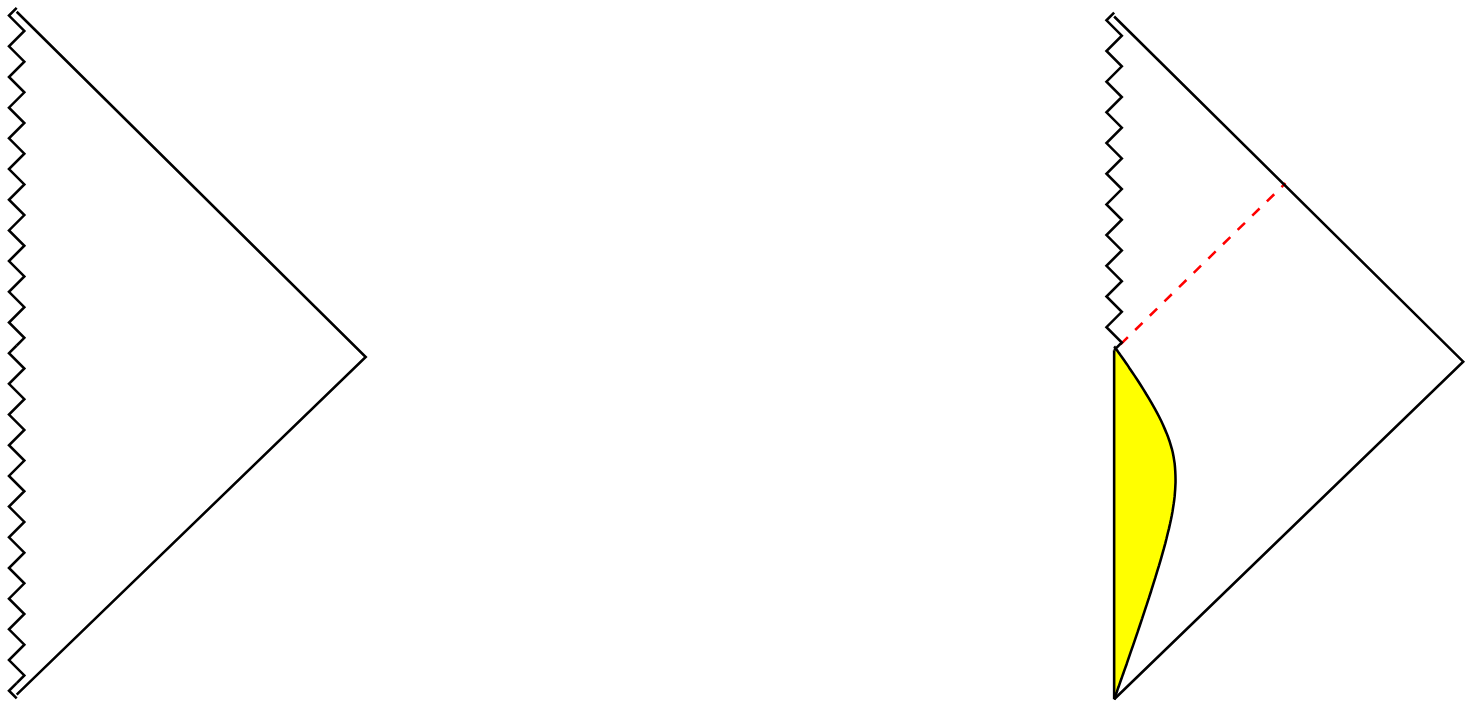
\includegraphics[width = 0.70 \textwidth]{cens-3.png}
  \caption{Penrose diagram for a negative mass black hole and unphysical collapse of a star.}
  \label{cens-3}
\end{figure}

An important conjecture in General Relativity, known as the \textit{weak cosmic censorship conjecture}, states the following: given matter which obeys the dominant energy condition Eq. \ref{eq:4.55}, generic smooth initial conditions on a spatial hypersurface for both the metric and matter fields in an asymptotically flat spacetime will not evolve to form naked singularities.\\
If this conjecture is true, then a dynamical evolution such as that in Fig. \ref{cens-3} must be ruled out: in this diagram, once the singularity forms, fields can no longer be evolved beyond the shown lightray; strictly speaking, this means that the dynamical evolution stops at the red line and cannot be extended further, thus abruptly ending $ \mathcal{I}^+ $.\\
There's no proof of the weak cosmic censorship conjecture, but only circumstantial evidence. However, there's one naked singularity that seems to be physical: the Big Bang singularity. In fact, since it is in the far past, it doesn't violate cosmic censorship.

\subsection{de Sitter black holes}

Schwarzschild metric Eq. \ref{eq:6.1} solves the Einstein field equations with $ \Lambda = 0 $, i.e. in asymptotically Minkowski spacetime. To generalize, consider $ \Lambda \neq 0 $, so that the field equations become $ R_{\mu \nu} = \Lambda g_{\mu \nu} $, and use the following (already seen) ansatz:
\begin{equation*}
  ds^2 = - f(r)^2 dt^2 + f(r)^{-2} dr^2 + r^2 \left( d\vartheta^2 + \sin^2 \vartheta \, d\varphi^2 \right)
\end{equation*}
The field equations imply that:
\begin{equation*}
  f'' + \frac{2f'}{r} + \frac{{f'}^2}{f} = - \frac{\Lambda}{f}
  \qquad \land \qquad
  1 - 2 f f' r - f^2 = \Lambda r^2
\end{equation*}
The most general solution is:
\begin{equation}
  f(r)^2 = 1 - \frac{2GM}{r} \mp \frac{r^2}{R^2}
  \qquad
  R^2 = \frac{3}{\abs{\Lambda}}
  \label{eq:6.14}
\end{equation}
where the negative sign is the solution with $ \Lambda > 0 $ and the positive sign with $ \Lambda < 0 $, hence describing black holes in de Sitter and anti-de Sidder spacetime respectively: in fact, if $ 2GM \ll R^2 $, then for $ r \ll R $ the metric is that of a Schwarzschild black hole in Minkowski spacetime.










